% !TEX root = ./main.tex
% Object-Oriented Languages
% ======================================================
\subsection*{Single Inheritance}

\begin{figure}[H]
    \centering
    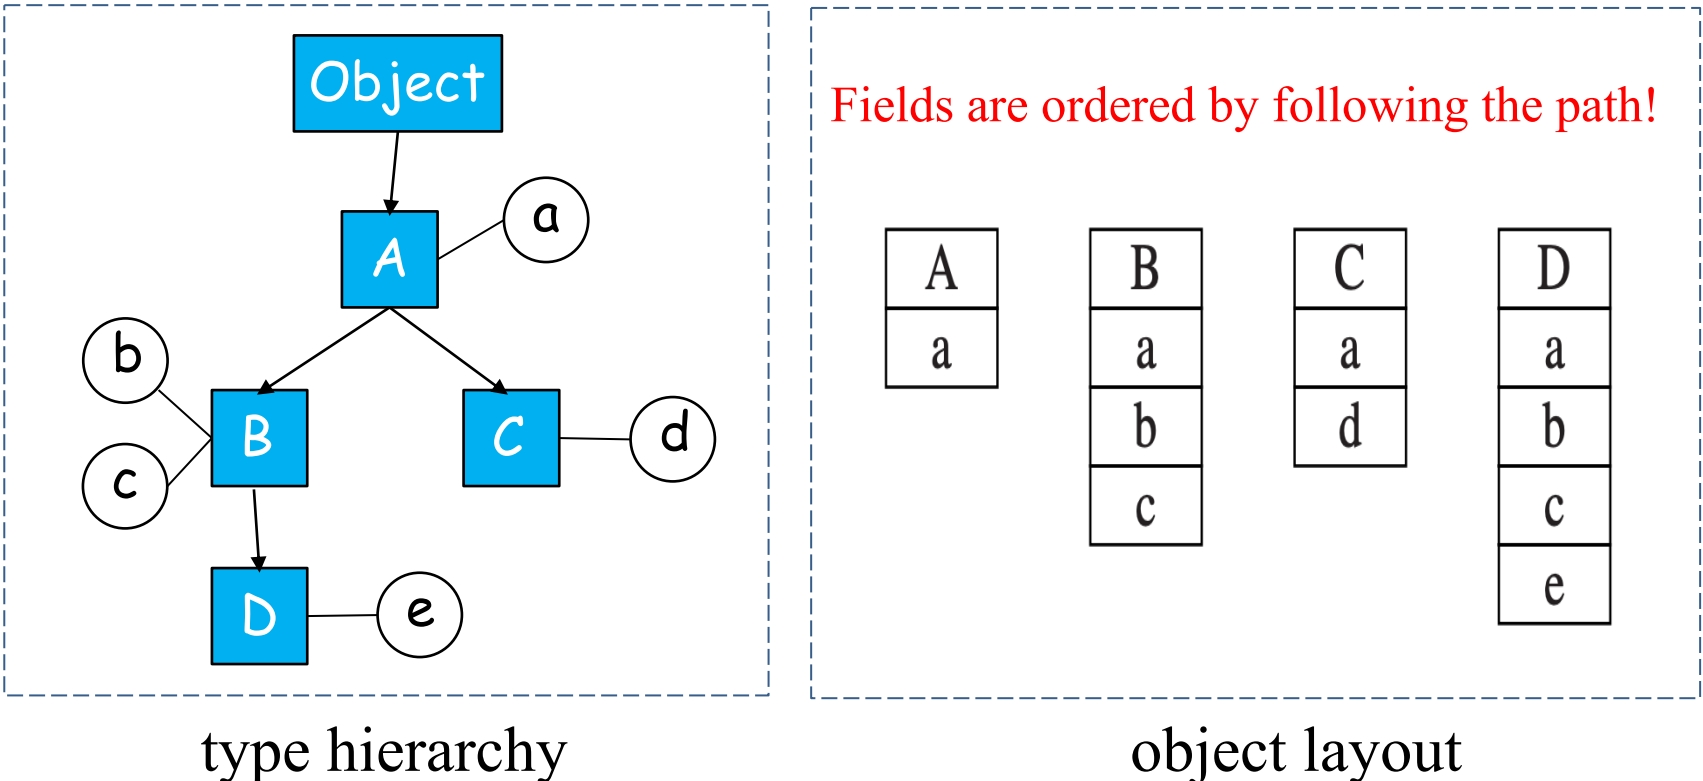
\includegraphics[width=0.40\linewidth]{figures/oop1.png}
    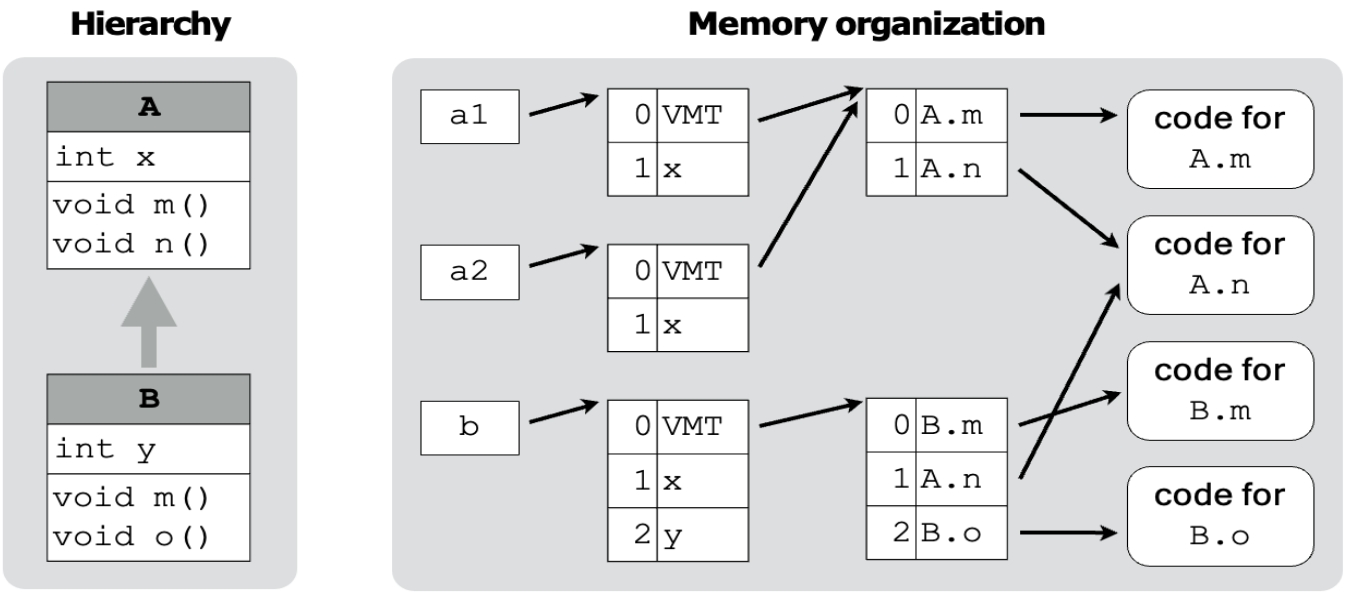
\includegraphics[width=0.58\linewidth]{figures/oop2.png}
\end{figure}

\par \noindent \textbf{Field layout}:继承的字段以相同的顺序放在类描述符头部。

\par \noindent \textbf{Method dispatch}(= generating method calls):每个类描述符都包含指向其父类的指针,以及方法实例列表。
\par \noindent 对于静态方法:调用 \texttt{c.f()} 时在类 C 中搜索方法 f,如果找不到 – 搜索 C 的父类,依此类推。
\par \noindent 对于动态方法:使用 dispatch vector(aka virtual table, vtable),记录所有方法的地址。
调用 \texttt{c.f()} 时从 c 中偏移量为 0 处获取类描述符 d,从 d 偏移 f (常数)中获取方法实例指针 p。

\subsection*{Multiple Inheritance}

\par \noindent \textbf{Field layout}:图着色算法,每个类的字段按照其在继承图中的位置着色,颜色代表其偏移量。
如果不同字段在同一个类型里出现了,那么它们就不能染成同一个颜色。优化:由于类型数远小于对象数,偏移量在类描述符中,而非直接在对象中。

\par \noindent \textbf{Method dispatch}:图着色算法,同上。

\par \noindent \textbf{Dynamic Linking Class}:无法使用图染色算法,解决方案是哈希表。
为每个类描述符构建哈希表:1. Ftab(字段表):包含字段偏移量和方法代码地址;2.Ktab(键表):包含字段/方法名称。
获取字段 b 的步骤:
1. 从偏移量 0 处获取类描述符;
2. 从 $\text{Ktab} + \text{hash}_b$ 处获取字段名;
3. 比较字段名和输入名;
4. 若相等,从 $\text{Ftab} + \text{hash}_b$ 处获取字段偏移量,假设为 $2$;
5. 从 $\text{object} + 2$ 处获取字段。

\par \noindent \textbf{Membership test}:每一个类描述符存储一个 display:类嵌套深度限制为某个常量(例:20),在每个类描述符中保留一个 20 字长的块。
给每个类指定一个数字标识符:

\begin{figure}[H]
    \centering
    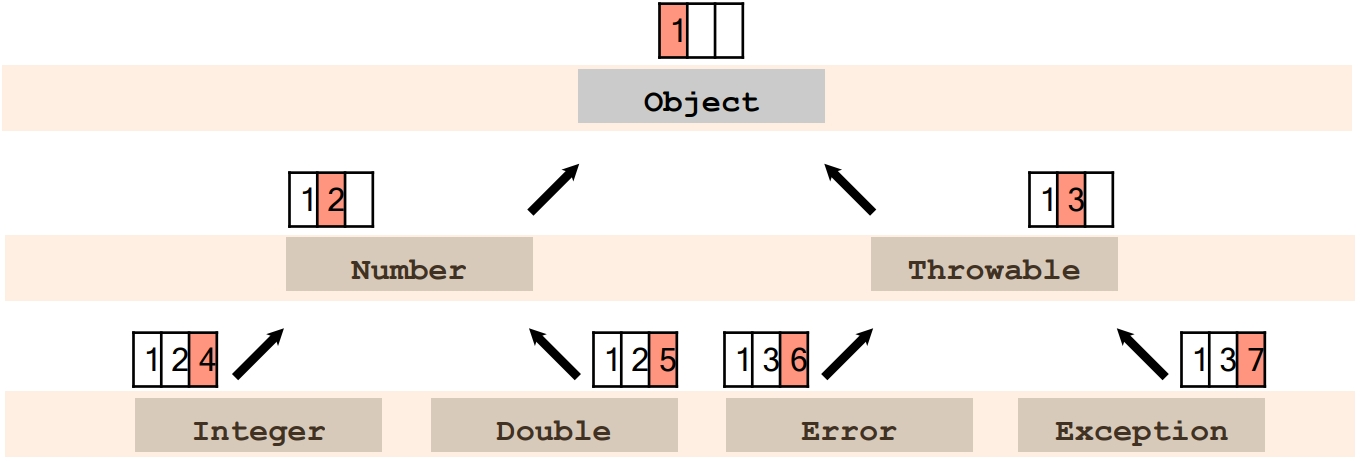
\includegraphics[width=0.8\linewidth]{figures/oop3.png}
\end{figure}

\par \noindent 通过类型检查可以实现私有方法/成员变量。类型转换到超类(upcast)是安全的,但是转换到子类(downcast)是不安全的。